
\section{Teori}

    \textbf{Motivasjon og sammenheng:} Målet er å få en dypere forståelse av hvordan elektriske signaler forplanter seg i ledningsnettverk. For å forstå utbredning av signaler i forskjellige transmisjonslinjer, bruker vi telegrafligningen. Denne beskriver hvordan elektriske signaler forplanter seg i transmisjonslinjer, og gir oss verktøyene til å analysere fenomener som demping, faseforskyvning og dispersjon. Dette er spesielt relevant for praktiske applikasjoner som Ethernet- og koaksialkabler, hvor signalets integritet over lengre avstander er avgjørende.

\subsection{Kirchhoffs lover}
Grunnlaget for telegrafligningen ligger i Kirchhoffs lover, som beskriver hvordan spenning og strøm 
fordeles i elektriske kretser. Disse lovene er direkte basert på fysikkens bevaringsprinsipper 
for energi og ladning, og de brukes til å beskrive forholdet mellom elektriske størrelser i ethvert 
kretsnettverk.
\subsubsection{Kirchhoffs spenningslov (KVL)} sier at summen av alle spenningsendringer rundt en lukket 
sløyfe er lik null. Dette uttrykker energibevaring: den elektriske energien som brukes opp i motstander 
og spoler, må være lik den energien som tilføres av spenningskilder. I telegrafligningen brukes KVL 
til å uttrykke hvordan spenningen endrer seg langs et lite element av ledningen. Spenningsfallet 
langs et element avhenger av den ohmske motstanden og induktansen, og beskrives matematisk som vist i ligningen \eqref{eq:KVL}.
\subsubsection{Kirchhoffs strømlov (KCL)} sier at summen av alle strømmene som går inn i et knutepunkt, 
er lik summen av de som går ut. Dette er et uttrykk for ladningsbevaring. I telegrafligningen brukes 
KCL til å beskrive hvordan strømmen endrer seg langs ledningen, når en del av strømmen lekker til jord 
gjennom konduktans og kapasitans. Dette gir ligningen \eqref{eq:KCL}.\\[1em]
Ved å kombinere Kirchhoffs lover kan man beskrive hvordan både spenning og strøm endrer seg 
langs ledningen over tid. Dette er utgangspunktet for telegrafligningen, som gir 
en fullstendig matematisk modell for hvordan signaler forplanter seg, dempes og forvrenges når de beveger 
seg gjennom en elektrisk leder.
\clearpage
\subsection{Fourier-rekker}

Mange signaler kan brytes ned i sine frekvenskomponenter ved hjelp av Fourier-analyse. Dette er spesielt nyttig i signalbehandling og for å forstå hvordan ulike frekvenser påvirkes av transmisjonslinjen. Ethernet-signaler kan sees på som en sekvens av pulser (bitstrøm), som i praksis kan betraktes som et periodisk pulstog. Dette gjør at Fourier-rekker er et naturlig verktøy for å analysere slike signaler i frekvensdomenet, siden pulstoget kan uttrykkes som en sum av sinus- og cosinuskomponenter.\\[1em]
En periodisk funksjon $f(t)$ med periode $T$ kan uttrykkes som en Fourier-rekke:
\begin{equation}
f(t) = a_0 + \sum_{n=1}^{\infty} \left( a_n \cos\left(\frac{2\pi n t}{T}\right) + b_n \sin\left(\frac{2\pi n t}{T}\right) \right)
\end{equation}
med koeffisienter gitt ved:
\begin{align*}
a_0 &= \frac{1}{T} \int_{0}^{T} f(t) \, dt \\
a_n &= \frac{2}{T} \int_{0}^{T} f(t) \cos\left(\frac{2\pi n t}{T}\right) dt \\
b_n &= \frac{2}{T} \int_{0}^{T} f(t) \sin\left(\frac{2\pi n t}{T}\right) dt
\end{align*}
I kompleks form:
\begin{equation}
f(t) = \sum_{n=-\infty}^{\infty} c_n e^{j \frac{2\pi n t}{T}}, \quad \text{der} \quad c_n = \frac{1}{T} \int_{-T/2}^{T/2} f(t) e^{-j \frac{2\pi n t}{T}} dt, \quad c_0 = \frac{1}{T} \int_{-T/2}^{T/2} f(t) dt
\end{equation}
I dette prosjektet modellerer vi en Cat5e-transmisjonslinje ved hjelp av Fourier-analyse
og en frekvensavhengig RLCG-modell. For et periodisk pulstog \(f(t)\) med periode \(T\)
(\(f_0=1/T\)) bruker vi Fourier-rekken \(\{c_n\}\) slik at hver harmoniske ved
\(f_n=nf_0\) kan analyseres separat. Hver komponent skaleres og fases av linjen gjennom
overføringsfunksjonen \(H(f)\). For en jevn linje med lengde \(\ell\) og korrekt terminering
gjelder:
\[
H(f)=e^{-\gamma(f)\,\ell},\qquad \gamma(f)=\alpha(f)+j\beta(f).
\]
Dermed er:
\[
H(f)=\frac{V_{\text{out}}(f)}{V_{\text{in}}(f)},\quad
V_{\text{out}}(f)=H(f)\,V_{\text{in}}(f).
\]
Som beskriver hvordan signalet endres i frekvensdomenet når det passerer gjennom kabelen.
Denne analysen hjelper oss å forstå hvordan ulike frekvenskomponenter dempes og forvrenges, noe som er avgjørende for å forklare begrensningen på kabelens lengde.
Setter vi inn overføringsfunksjonen i komplekse Fourier-rekken, kan vi modellere hvordan hele signalet endres når det går gjennom kabelen \cite{engineering_mathematics}.
\begin{equation}
    f_{out}(t) = \sum_{n=-\infty}^{\infty} H\left(\frac{n}{T}\right) c_n e^{j \frac{2\pi n t}{T}}
\end{equation}
\clearpage
\subsection{Telegrafligningen og transmisjonslinjer}
En transmisjonslinje kan beskrives ved fire per-enhet-lengde parametre:
\begin{itemize}
    \item $R$ \, [$\Omega$/m] \,-- Motstand (ledertap),
    \item $L$ \, [H/m] \,-- Induktans (magnetisk lagring),
    \item $C$ \, [F/m] \,-- Kapasitans (elektrisk lagring),
    \item $G$ \, [S/m] \,-- Konduktans (lekkasjetap).
\end{itemize}
Ved å kombinere Kirchhoffs lover med disse parameterne utledes telegrafligningen, som beskriver spenning og strøm som funksjon av både posisjon og tid langs kabelen. For spenningen $u(x,t)$ kan den skrives på formen:
\begin{equation}
    u_{tt} + \left(\frac{R}{L} + \frac{G}{C}\right)u_t + \left(\frac{RG}{LC}\right)\,u = \left(\frac{1}{LC}\right) u_{xx}
\end{equation}
der $u(x,t)$ er spenningen langs kabelen og $c$ er utbredelseshastigheten i kabelen.  
Denne ligningen viser at et signal ikke bare forplanter seg med en hastighet bestemt av $L$ og $C$, men også blir dempet og forvrengt på grunn av $R$ og $G$. Resultatet er at høyfrekvente komponenter i signalet svekkes og spres mer enn lave frekvenser, noe som over tid fører til \emph{demping og dispersjon}.  
Ethernet-signaler består ikke av rene sinusbølger, men av pulser med et bredt spekter av frekvenser. Mens Fourier-analyse kan hjelpe oss  å uttrykke signalet som en sum av ulike frekvenskomponenter, gir telegrafligningen oss verktøy til å studere hvordan hver enkelt komponent påvirkes. Dermed kan vi forklare hvorfor en grense på omtrent 100m er praktisk: etter denne lengden er tapet og forvrengningen så store at signalet ikke lenger kan tolkes pålitelig for mottakeren.


\subsubsection{R - Resistans}
Resistans per lengde $[\Omega/\mathrm{m}]$ er den ohmske motstanden i lederen. Den skyldes av materialets resistivitet og ledertverrsnitt, og øker med temperatur. Motstanden øker dempingen og reduserer rekkevidden til signalet. I telegrafligningen bidrar R direkte til tidsdemping av både strøm og spenning.

\subsubsection{L - Induktans}
Induktansen per lengde $[\mathrm{H}/\mathrm{m}]$ er magnetisk lagring av energi rundt lederen når strømmen endres, per meter kabel. Sammen med kapasitans vil denne bestemme farten på signalet i kabelen. I linjemodellen står induktansen i serie.

\subsubsection{C - Kapasitans}
Kapasitans per lengde $[\mathrm{F}/\mathrm{m}]$ er elektrisk lagring av energi i feltet mellom leder og referanse, per meter. Sammen med induktans har kapasitans påvirkning på fart. I linjemodellen er dette en gren til jord, den trekker ladning når spenningen endres.

\subsubsection{G -- Konduktans per lengdeenhet (lekkasje)}
$G$ [$\mathrm{S/m}$] er \textit{konduktansen per lengdeenhet} til jord, ofte kalt 
\textit{shunt-konduktansen}. Den modellerer lekkasjestrøm gjennom kabelens isolasjon og står 
parallelt med kapasitansen $C$ i den ekvivalente linjemodellen. En større $G$ gir økt demping 
fordi mer energi går tapt i dielektrikumet. 
\\[1em]
Verdien av $G$ avhenger av materialets kvalitet og miljøforhold: høy fuktighet, aldring eller 
skadet isolasjon øker $G$, mens ideell isolasjon gir $G \approx 0$. Parameteren beskriver dermed 
tap som skyldes ufullkommen isolasjon mellom lederen og jord.
\subsubsection{Utledning av telegrafligningen}
Telegrafligningen kan utledes ved å analysere en liten del av transmisjonslinjen, som vist i figuren nedenfor. Vi betrakter et segment av linjen med lengde $\Delta x$,  og bruker Kirchhoffs spennings- og strømlov for å sette opp differensialligninger for spenning og strøm \cite{TelegraflikningenPDF}.
\begin{figure}[h]
    \centering
    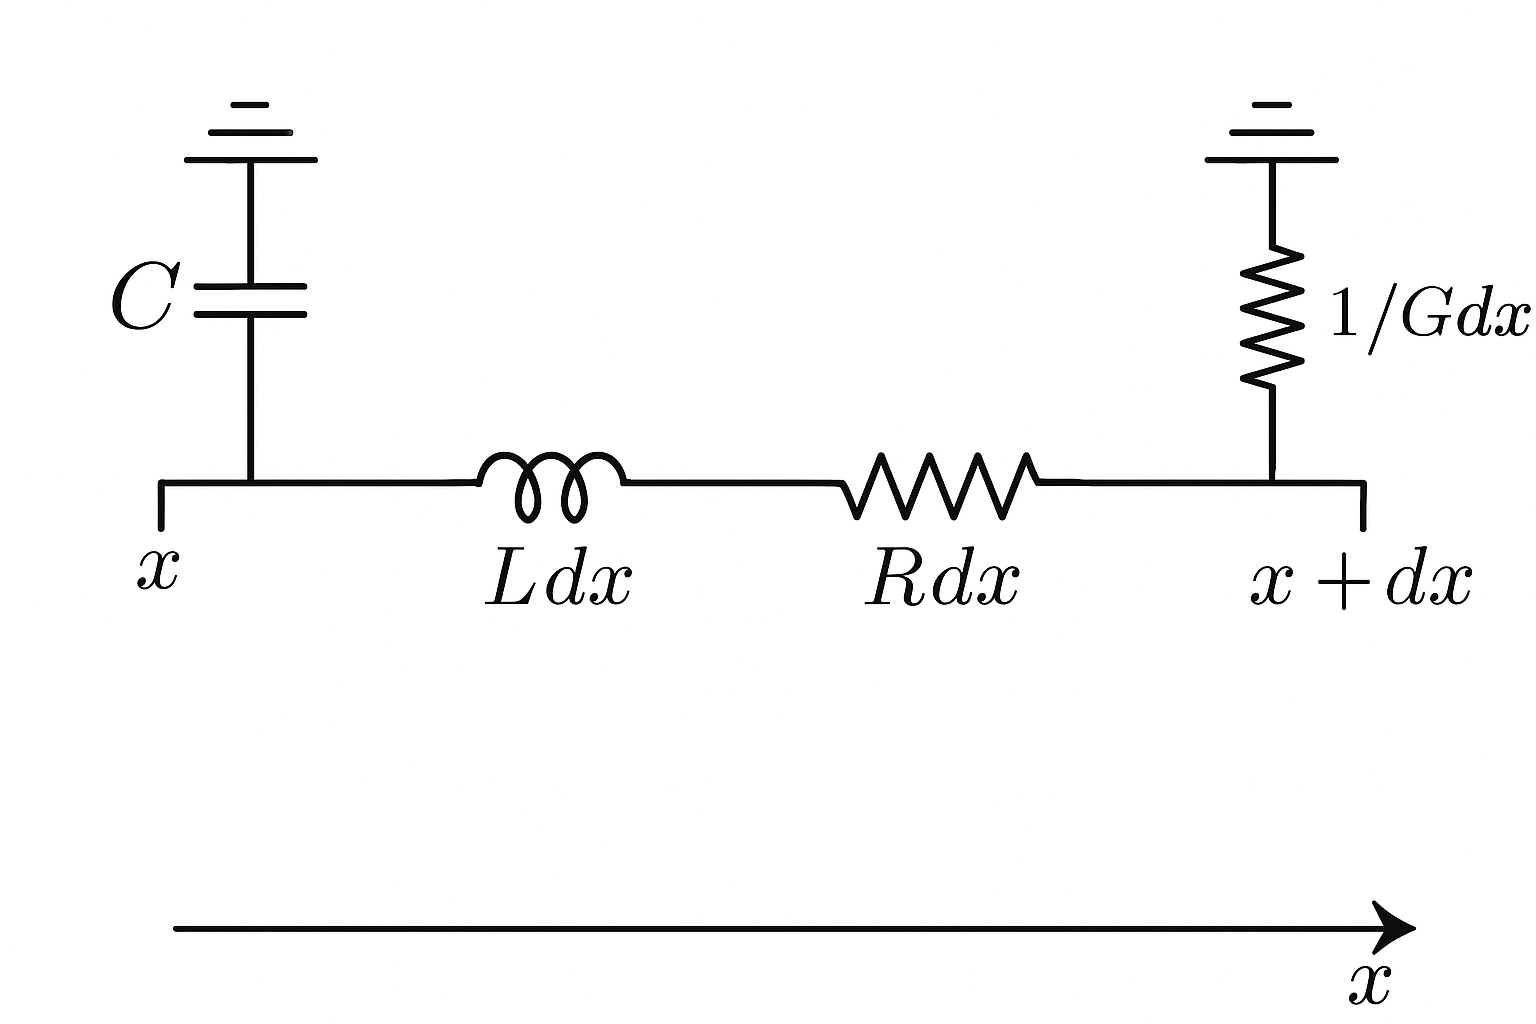
\includegraphics[width=0.6\textwidth]{Media/telegraflinje.png}
    \textit{
        \caption{Elementært segment av en transmisjonslinje med per-enhet-lengde parametere \cite{TelegraflikningenPDF}.}\label{fig:transmission_line_segment}   }
    
\end{figure}\\
Ved å anvende Kirchhoffs spenningslov på segmentet får vi:
\[
    u(x,t) - u(x+\Delta x,t) = R \Delta x \cdot i(x,t) + L \Delta x \cdot \frac{\partial i(x,t)}{\partial t} .
\]
Når man deler begge sider av ligningen på $\Delta x$ og lar $\Delta x \to 0$, får vi uttrykket for spenningsendringen:
\begin{equation}
    \frac{\partial u(x,t)}{\partial x} = -R i(x,t) - L \frac{\partial i(x,t)}{\partial t}.
    \label{eq:KVL}
\end{equation}
\\Tilsvarende, ved å bruke Kirchhoffs strømlov, får vi:
\[
    i(x,t) - i(x+\Delta x,t) = -G \Delta x \cdot u(x,t) - C \Delta x \cdot \frac{\partial u(x,t)}{\partial t} .
\] 
\begin{equation}
    \frac{\partial i(x,t)}{\partial x} = -G u(x,t) - C \frac{\partial u(x,t)}{\partial t}.
    \label{eq:KCL}
\end{equation}
Ved å kombinere disse to relasjonene, ved å derivere den første med hensyn på $x$ og den andre med hensyn på $t$, og deretter eliminere $i(x,t)$, får vi telegrafligningen for spenningen:
\[
    u_{tt} + \left(\frac{R}{L} + \frac{G}{C}\right)u_t + \left(\frac{RG}{LC}\right)\,u = \left(\frac{1}{LC}\right) u_{xx}
\]
\clearpage
\noindent Dette kan vi skrive som:
\begin{equation}
    u_{tt} + (\aH + \bH)u_t + \aH \bH u = c^2 u_{xx},\quad (i \ tapsfri\ linje: c = \frac{1}{\sqrt{LC}}).
    \label{eq:telegraflikningen}
\end{equation}
der vi definerer:
\[
    \aH = \frac{R}{L}, \qquad \bH = \frac{G}{C} .
\]
Dette er en dempet bølgeligning som beskriver hvordan spenningen forplanter seg langs transmisjonslinjen, med demping og forvrengning bestemt av parametrene $RLCG$.
\subsection{Propagerende løsning og overføringsfunksjon}

I forrige del utledet vi telegrafligningen for spenning langs en kabel uttrykt ved de per-lengde-parametrene $RLCG$ som beskriver hvordan spenningen varierer både i tid og rom \eqref{eq:telegraflikningen}. Denne likningen er en såkalt bølgelikning med demping. Vi forventer derfor at løsningene skal ha bølgekarakter som oscillerer i tid og samtidig forplanter seg langs kabelen. For å fange dette opp antar vi en løsning på formen \cite{HaytBuck2018}
\begin{equation}
v(x,t) = \Re\!\left\{ U e^{j\omega t - \gamma(\omega)x} \right\}.
\label{eq:harm-ansatz}
\end{equation}
Her har vi valgt tre elementer:
\begin{itemize}
    \item \textbf{Tidsdelen $e^{j\omega t}$:} beskriver en harmonisk oscillasjon i tid. At vi bruker den 
    komplekse eksponentialen i stedet for $\cos(\omega t)$ eller $\sin(\omega t)$ skyldes at dette 
    gjør beregningene enklere. Til slutt tar vi realdelen for å hente ut det fysiske signalet.\\
    \item \textbf{Romdelen $e^{-\gamma x}$:} beskriver hvordan signalet utvikler seg langs kabelens lengde. 
    Hvis $\gamma$ er reell, betyr dette ren demping. Hvis $\gamma$ er imaginær, betyr det ren faseforskyvning. 
    I praksis er $\gamma$ kompleks, slik at vi får begge deler.\\
    \item \textbf{Kompleks amplitude $U$:} setter størrelsen og fasen på bølgen.\\
\end{itemize}
Dette kalles en \emph{harmonisk ansats}. Den er valgt fordi vi vet fra Fourier-teori at alle signaler 
kan bygges opp som en sum av slike harmoniske komponenter. Når vi kjenner kabelens respons på en frekvens, 
kan vi utvide til vilkårlige signaler. Setter vi \eqref{eq:harm-ansatz} inn i telegrafligningen \eqref{eq:telegraflikningen}:
\[    
    v_{tt} + (\aH + \bH)v_{t} + \aH \bH v = c^2 v_{xx}.
\]
Ser vi at den tidslige avledningen bare gir faktorer av $j\omega$:
\[
    v_{t} = j\omega v, \quad v_{tt} = -\omega^2 v,
\]
og den romlige avledningen gir faktorer av $\gamma$:
\[
    v_{x} = -\gamma v, \quad v_{xx} = \gamma^2 v.
\]
Som gir oss:
\[    
-\omega^2 v + j\omega(\aH+\bH)v + \aH \bH v = c^2 \gamma^2 v.
\]
Vi kan forkorte med $v$ (som er forskjellig fra null) og får:
\[
c^2 \gamma^2(\omega) = \aH \bH - \omega^2 + j\omega(\aH+\bH).
\]
\clearpage
\noindent Dette er en såkalt \emph{dispersjonsrelasjon}, som forteller hvilke kombinasjoner av 
frekvens $\omega$ og bølgetall $\gamma$ som er mulige. Vi kan løse for $\gamma$ og får:
\[
\gamma(\omega) = \frac{1}{c}\sqrt{\aH\bH - \omega^2 + j\omega(\aH+\bH)}.
\]
Setter vi inn definisjonene på $\aH,\bH$ og $c$, kan dette skrives på den standardformen
som brukes i transmisjonslinjeteori:
\begin{equation}
\;\gamma(\omega) = \sqrt{(R+j\omega L)(G+j\omega C)}\;
\label{eq:prop-konstant}
\end{equation}
Dette uttrykket viser tydelig hvordan både ledertap ($R$) og dielektriske tap ($G$) bidrar 
til at signalet dempes, mens $L$ og $C$ bestemmer hastigheten til bølgen. Vi kan også uttrykke $\gamma$
i form av sin reelle og imaginære del:
\[
\gamma(\omega) = \alpha(\omega) + j\beta(\omega).
\]
Her har $\alpha(\omega)$ enheten Np/m (neper per meter) og forteller hvor raskt amplituden 
avtar med lengden, mens $\beta(\omega)$ har enheten rad/m og forteller hvor raskt fasen 
øker langs kabelen. Fra $\beta$ kan vi utlede bølgens fasehastighet:
\[v_p = \frac{\omega}{\beta}\]
og dermed hvor stor tidsforsinkelse signalet får etter en viss lengde.\\[1em]
Hvis vi nå ser på en kabel av lengde $\ell$, vil en harmonisk komponent ved frekvens $\omega$ 
endres med faktoren:
\begin{equation}
H(\omega,\ell) = e^{-\gamma(\omega)\ell} = e^{-\alpha(\omega)\ell}\,e^{-j\beta(\omega)\ell}
\end{equation}
Dette er kabelens \emph{overføringsfunksjon} \cite{wikipedia_telegrapher}. 
Den kan forstås slik:
\begin{itemize}
    \item \textbf{$e^{-\alpha \ell}$}: amplituden reduseres eksponentielt med lengden, 
    \item \textbf{$e^{-j\beta \ell}$}: signalet forskyves i fase, tilsvarende en tidsforsinkelse.\\[1em]
\end{itemize}
Så langt har vi bare sett på en harmonisk bølge. Men i praksis er alle signaler satt sammen av mange slike bølger. 
Et vilkårlig innsignal kan skrives som en Fourier-rekke:
\[
f_{\text{in}}(t) = \sum_n c_n e^{j\omega_n t}.
\]
Etter kabelen vil hver komponent være påvirket av $H(\omega_n,\ell)$, og vi får:
\[
f_{\text{out}}(t) = \sum_n H(\omega_n,\ell)\,c_n e^{j\omega_n t}.
\]
Dermed virker kabelen som et frekvensavhengig filter: lave frekvenser slipper nesten uendret gjennom, 
mens høye frekvenser dempes kraftig. For firkantsignaler betyr dette at de skarpe kantene, 
som består av mange høye frekvenser, gradvis blir avrundet etter hvert som lengden øker. 
Det er nettopp dette vi kan observere i laboratoriet når vi sender firkantpulser gjennom en Ethernet-kabel.



\clearpage
\subsubsection{Demping (amplituderespons)}
Demping beskrives av realdelen av propagasjonskonstanten \cite{HaytBuck2018}:
\[ 
  \alpha(\omega)=\Re\{\gamma(\omega)\}
\]
Den sier noe om hvor stor faktor hver frekvenskomponent dempes i amplitude. Denne faktoren er definert som størrelsen av overføringsfunksjonen:
\[
|H(\omega,\ell)|=e^{-\alpha(\omega)\,\ell}, \qquad |H(\omega,\ell)|_{\mathrm{dB}} = 20\log_{10}|H| = -8.686\,\alpha(\omega)\,\ell
\]
Når $c_n$ er Fourier-koeffisienten til n-te harmoniske komponent, er amplituden til denne komponenten etter kabelen gitt ved:
\[
|c_n^{out}| = |H(\omega_n,\ell)| \cdot |c _n| = e^{-\alpha(\omega_n) \ell} |c_n|
\]
Hvorfor signalet dempes kan forklares med to hovedmekanismer:\\
\begin{itemize}[leftmargin=2.8em,style=nextline]
  \item \textbf{Skinneffekt}: Når frekvensen øker, presses strømmen mot overflaten av lederen. Det effektive tverrsnittet blir mindre, og den elektriske motstanden per lengde øker. For runde ledere (og godt approksimert i praksis) gjelder :
    \begin{equation}
        R(\omega) = R_{DC} \cdot \sqrt{\frac{\omega}{\omega_{s}}}, \quad hvor \quad \omega_{s} = \frac{2 \rho}{ \mu r^2}, \quad R_{DC} = n_s \cdot \frac{\rho}{\pi r^2}
        \label{eq:skin-effekt}
    \end{equation}
    Her er $\omega_{s}$ den skinneffektsfaktoren for runde ledere, $R_{DC}$ den DC motstanden per meter, $n_s$ tar hensyn til antall ledere i serie (2 for tvinnet par), $\rho$ er resistiviteten til lederen, $\mu$ er permeabiliteten til lederen og $r$ er radiusen til lederen \cite{PalermoLecture2023}. Vi ser dermed at:
    \[
    R(\omega)\ \propto\ \sqrt{\omega}
    \]
  Ut fra propagasjonskonstanten \eqref{eq:prop-konstant} følger at $\alpha(\omega)$ vokser omtrent som $\sqrt{\omega}$.\\
  \item \textbf{Dielektriske tap}: Et virkelig dielektrikum er ikke tapsfritt: polarisasjonen henger litt etter feltet (faseforsinkelse), noe som kan modelleres med \emph{loss tangent} \(\tan\delta\). For små tap får vi den nyttige tilnærmingen:
  \begin{equation}
  G(\omega)\ =\ \omega\,C\,\tan\delta \quad \Rightarrow \quad G(\omega)\ \propto\ \omega
    \label{eq:dielectric_loss}
  \end{equation}
  slik at tapet øker lineært med frekvens. Dette bidrar også til \(\alpha(\omega)\) og dermed til økende demping med \(\omega\) \cite{PalermoLecture2023}.\\
\end{itemize}
\clearpage

\noindent Dette gir da direkte utslag i overføringsfunksjonen. Siden både \(R(\omega)\) og \(G(\omega)\) øker med frekvens, dempes høyfrekvente komponenter mest.
I tid betyr det sløvere kanter og “droop” på platået (vertikal lukking i øyediagram) siden høye frekvenser som trengs for å gjenskape skarpe kanter, er mest dempet.
\begin{figure}[h]
    \centering
    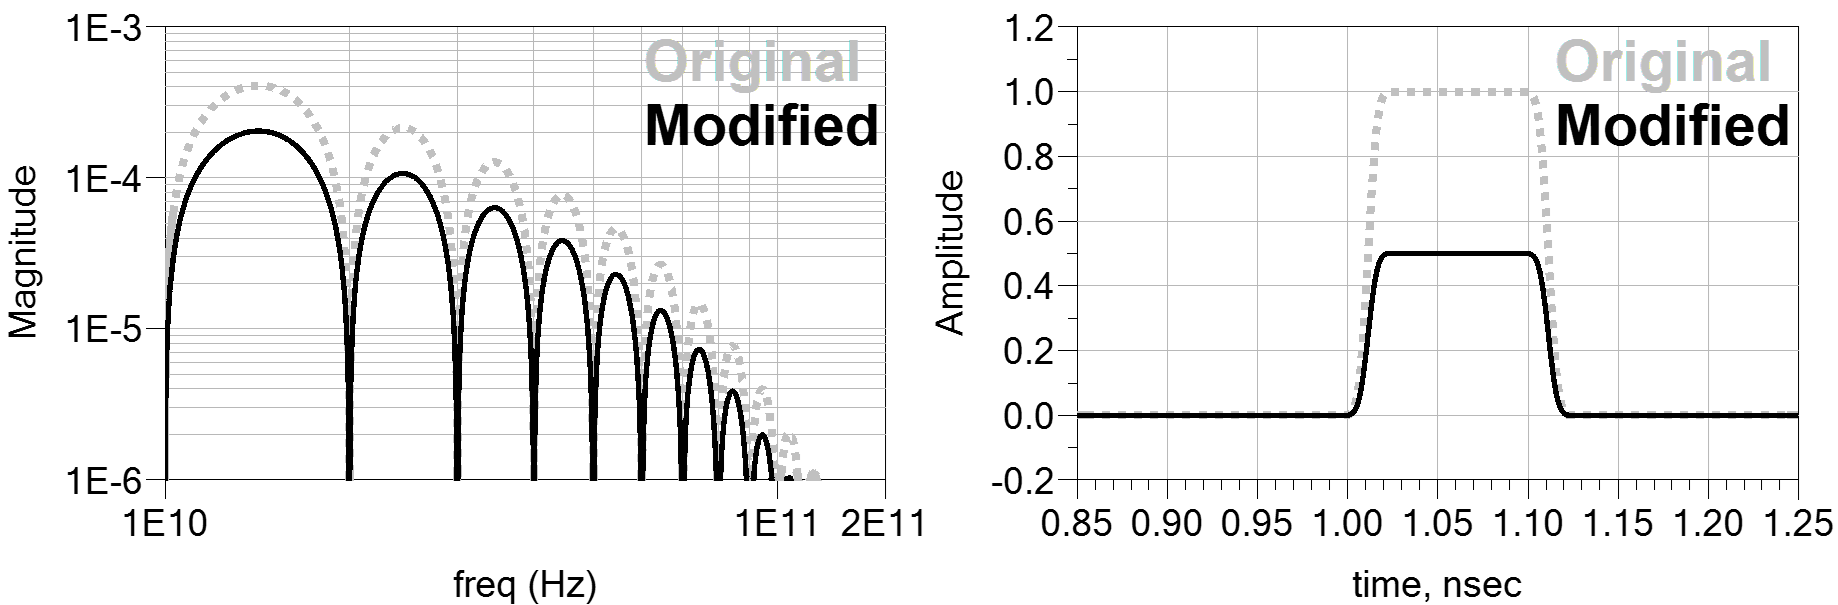
\includegraphics[width=0.9\textwidth]{Media/frekvensdoment_tidsdoment.png}
    \textit{
        \caption{Tids- og frekvensdomene av original og modifisert bølgeform. Pulsformen bestemmes av forholdet mellom frekvenskomponentene; er amplituder og relative faser like, blir tidskurven uendret \cite{figure2}.}\label{fig:eyediagram}}
    
\end{figure}
\subsubsection{Dispersjon (fase, gruppeforsinkelse og gruppehastighet)}
Dispersjon beskrives av den imaginære delen av propagasjonskonstanten (fasekonstanten) \cite{HaytBuck2018}:
\[
    \beta(\omega)=\Im\{\gamma(\omega)\}
\]
Den sier noe om hvor mye hver frekvenskomponent forskyves i fase.
Fasen til kabelen er gitt ved:
\[
\varphi(\omega,\ell) = -\beta(\omega)\,\ell
\]
Fra fasen kan vi finne \emph{gruppeforsinkelse} og \emph{gruppehastighet}.
\emph{Gruppeforsinkelse} er definert som:
\[
\tau_g(\omega,\ell) = \varphi'(\omega,\ell) = -\frac{d}{d\omega}\varphi(\omega,\ell) = \ell\,\frac{d\beta(\omega)}{d\omega}
\]
Den sier noe om hvor mye en smal båndbredde rundt frekvensen \(\omega\) forsinkes i tid etter å ha passert kabelen. \emph{Gruppehastighet} er definert som:
\[
v_g(\omega) = \frac{1}{\tau_{g}'(\omega)} = \left(\frac{d\beta(\omega)}{d\omega}\right)^{-1}, \quad hvor \quad \tau_g'(\omega) = \frac{\tau_g(\omega,\ell)}{\ell} = \frac{d\beta(\omega)}{d\omega} \quad [\mathrm{s/m}]
\]
\noindent Den sier noe om hvor raskt en smal båndbredde rundt frekvensen \(\omega\) forplanter seg i kabelen. Det vi ser her er at \(\tau_g\) og \(v_g\) avhenger av frekvensen og det er nettopp dette som kalles \emph{dispersjon}. Vi kan tolke dette slik at ulike frekvenskomponenter av et signal forplanter seg med ulik hastighet. 
\clearpage
\noindent Dette får direkte konsekvenser for pulsform og øyediagram.\\
\begin{itemize}[leftmargin=2.8em,style=nextline]
  \item \textbf{Ingen dispersjon:} Hvis \(\frac{d\beta}{d\omega} \) er konstant (lineær fase), får alle frekvenskomponenter samme tidsforsinkelse \(\Rightarrow\) ingen pulsbredding (ingen horisontal øyelukking).\\
  \item \textbf{Dispersjon:} Når \(\frac{d\beta}{d\omega}\) varierer med frekvens (ikke-lineær fase), får ulike frekvenskomponenter ulik tidsforsinkelse \(\Rightarrow\) pulsbredding (horisontal øyelukking). I lavtap-tilfellet er ofte 
  \[
    \beta(\omega)\approx \omega\sqrt{LC}\quad,\quad slik\quad at \quad \tau_{g}'(\omega)=\frac{d\beta}{d\omega}\approx \sqrt{LC}\quad,\quad v_g(\omega)\approx \frac{1}{\sqrt{LC}}
  \]
  (nær konstant): da blir formen mest påvirket av demping, ikke fase-dispersjon.\\
\end{itemize}
\textbf{Spesialtilfelle (forvrengningsfri linje):}\\
Heaviside-betingelsen:
\[
    \aH = \bH \quad \Rightarrow \quad \frac{R}{L}=\frac{G}{C}
\]
gir \(\beta(\omega)\) lineær i \(\omega\)
(konstant \(\tau_g'\)) og \(\alpha(\omega)\) frekvensuavhengig. Da fås ingen dispersiv forvrengning (kun lik demping av alle frekvenser).
\subsubsection{Kobling til pulstog}
Et periodisk innsignal med Fourierkoeffisienter \(c_n\) filtreres som
\[
f_{\text{out}}(t)=\Re\!\left\{\sum_{n=-N}^{N} c_n\,H(\omega_n,\ell)\,e^{j\omega_n t}\right\}.
\]
Demping (via \(\alpha\)) fjerner spesielt de høye leddene \(\Rightarrow\) langsommere kanter.\\
Dispersjon via: 
\[\frac{d\beta}{d\omega}\] 
tidsforskyver leddene relativt \(\Rightarrow\) pulsbredding.
\subsection{Karakteristisk impedans}
En transmisjonslinjes karakteristiske impedans \(Z_0\) er definert som forholdet mellom spenning og strøm for en bølge som forplanter seg langs linjen uten refleksjoner \cite{HaytBuck2018}. Den er gitt ved:
\[
Z_0(\omega) = \sqrt{\frac{R + j\omega L}{G + j\omega C}} = \frac{V_0^+}{I_0^+} 
\]
Her er \(V_0^+\) og \(I_0^+\) amplitudene til den fremadgående spenningen og strømmen.
Denne impedansen er generelt kompleks og frekvensavhengig, noe som betyr at både resistive (RG) og reaktive komponenter (LC) påvirker signalet. 
\clearpage
\noindent For høye frekvenser, hvor \(j\omega L\) og \(j\omega C\) dominerer over \(R\) og \(G\), nærmer den karakteristiske impedansen seg:
\[
    R \ll \omega L, \quad G \ll \omega C \quad \Rightarrow \quad Z_0(\omega) \approx \sqrt{\frac{L}{C}}
\]
Dette er den ideelle karakteristiske impedansen for en tapsfri linje. I praksis må transmisjonslinjer ofte matches til kildens og lastens impedans for å minimere refleksjoner som gir stående bølger. Refleksjonskoeffisienten ved en last er gitt ved:
\[
    \Gamma = \frac{Z_L - Z_0}{Z_L + Z_0}, \quad hvor \quad Z_L \quad er \quad lastimpedansen.
\]
\[
    Z_0 = Z_L, \quad \Rightarrow \quad \Gamma = 0 \quad (ingen\ \ refleksjon)
\]
Om vi har en mismatch, vil vi få en løsning som er en superposisjon av frem- og tilbakegående bølger gitt ved:
\[
    v(x,t) = \Re\!\left\{ U_+ e^{j\omega t - \gamma x} + U_- e^{j\omega t + \gamma x} \right\}, \quad hvor \quad U_- = \Gamma U_+
\]
\noindent Noe som kan føre til interferens og forvrengning av signalet. Dette er spesielt kritisk i høyfrekvente applikasjoner som RF- og mikrobølgekommunikasjon, hvor selv små refleksjoner kan ha betydelig innvirkning på signalintegriteten. Derfor er det viktig å designe transmisjonslinjer med riktig karakteristisk impedans og å bruke passende termineringer for å sikre optimal ytelse.
Ulike typer kabler, som koaksialkabler og tvinnede par, har forskjellige karakteristiske impedanser basert på deres fysiske konstruksjon og materialegenskaper. Ethernet-kabler har typisk en karakteristisk impedans på 100\(\Omega\), mens koaksialkabler ofte har $50\Omega$ eller $75\Omega$. I modellering antar vi at kabelen er korrekt terminert med sin karakteristiske impedans for å unngå refleksjoner og stående bølger.
\subsection{Koaksialkabelen (brukt i lab) som transmisjonslinje}
En koaksialkabel er en praktisk realisering av transmisjonslinjemodellen. Den består av en indre leder omgitt av et isolerende dielektrikum og en ytre leder som fungerer som skjerm. Denne oppbygningen gir god skjerming mot elektromagnetisk støy og jevn feltfordeling, noe som gjør kabelen egnet for høyfrekvente signaler. I laboratoriet brukes koaksialkabler for å undersøke hvordan signaler dempes og forvrenges over lengde.
\subsection{Oppsummering og kobling til prosjektet}
Teorien forklarer hvorfor signaler i lange kabler dempes og forvrenges, og gir oss verktøyene til å analysere dette både analytisk og numerisk. Dette kan gi oss innsikt i hvorfor det er en anbefalt grense på 100m for Ethernet-kabler og hvordan koaksialkabler av forskjellige lengder påvirker signalet i frekvensdomenet. I det videre arbeidet skal vi gjennomføre numeriske simuleringer og praktiske målinger, slik at vi kan modellere effekten av demping og dispersjon på signaler i kabler numerisk og bruke måledata til å validere prinsippene.
